
\chapter{Methodology}
\begin{refsection}
 
This chapter presents the systematic methodology that will be employes to develop and evaluate the Retrieval-Augmented Generation (RAG)- based Large Language Model (LLM) chatbot system for literature search and thesis retrieval in the CSPC Library. The methodology includes the research design, theoretical and mathematical framework, software and hardware tools, instruments, procedures, evaluation metrics, and a conceptual framework.

\section{Research Design}

This study will adopt a \textit{constructive research approach}, which focuses on designing and building technological artifacts to address real-world problems and evaluating their practical utility \citeauthor{lukka2003cons} \citeyear{lukka2003cons}. This methodology is particularly well-suited to fields like information systems and artificial intelligence, where the goal is not only theoretical insight but also the creation of innovative, functional systems.

In this research, the primary artifact will be a \textit{Retrieval-Augmented Generation (RAG)}-based chatbot integrated with a \textit{Large Language Model (LLM)}. The system is designed to streamline thesis and literature retrieval within the CSPC Library by enabling semantically meaningful interactions between students and academic documents. 

The system will incorporate the functionalities of:

\begin{samepage}
\begin{itemize}
    \item CSPC email authentication for user verification
    \item Semantic search using vector embeddings
    \item Query history tracking for improved user experience
    \item Retraining support to adapt to future academic datasets
\end{itemize}
\end{samepage}


These features highlight the system's real-world relevance, sustainability, and potential for long-term utility \cite{hevner2004design}.

The system will be developed using Streamlit, which allows rapid deployment of an interactive user interface. The backend combines vector databases and transformer-based LLMs, demonstrating how retrieval and generation components can be effectively integrated to improve access to academic resources.

\section{Theorems, Algorithms, and Mathematical Models}

This study will implement advanced machine learning techniques, natural language processing (NLP) models, and the Retrieval-Augmented Generation (RAG) pipeline, integrated with a Large Language Model (LLM) and a vector database. These components will collaboratively enable efficient information retrieval and generation in the context of literature and thesis search within the CSPC Library.

\newpage
\clearpage
\subsection{Retrieval-Augmented Generation (RAG) Pipeline}

The Retrieval-Augmented Generation (RAG) pipeline is a hybrid architecture that combines information retrieval with natural language generation. It allows LLMs to access external documents during inference, thereby improving both accuracy and contextual relevance.

\begin{figure}[htbp]
    \centering
    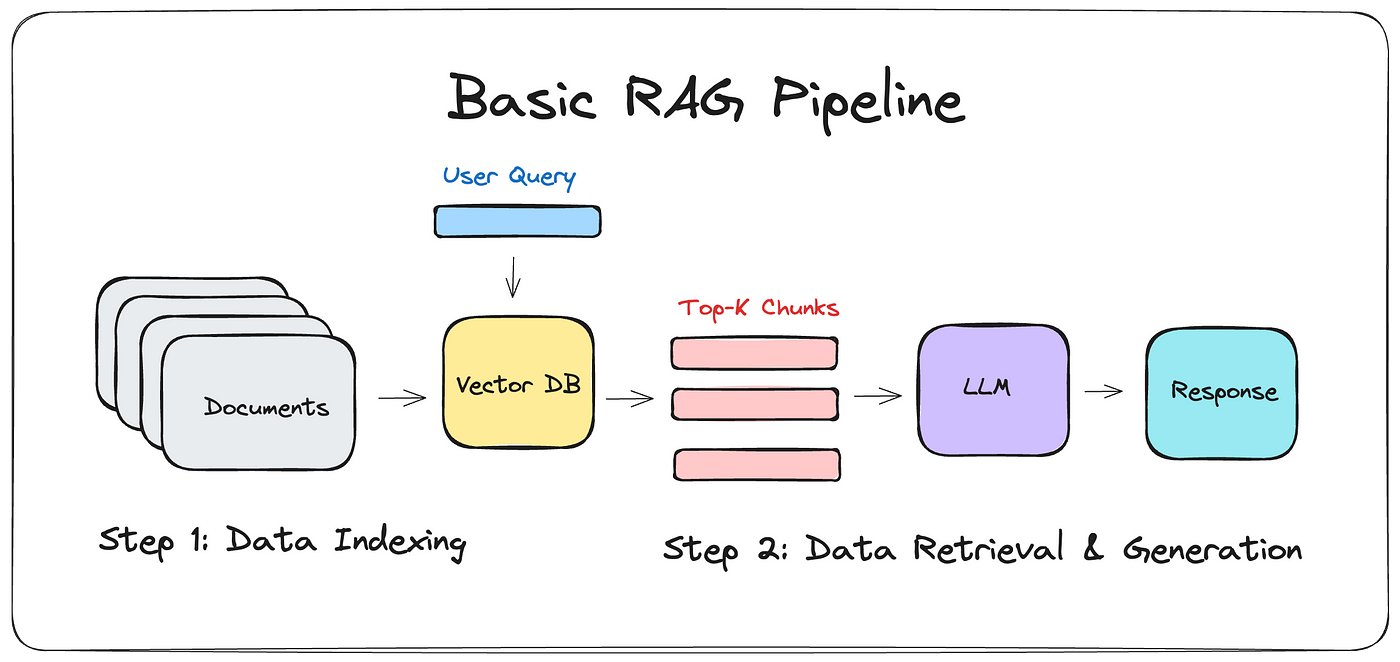
\includegraphics[width=0.7\textwidth]{figures/rag.png}
    \caption{Basic RAG Pipeline by Dr. Julija}
    \label{fig:rag}
\end{figure}

The chatbot’s RAG pipeline, as illustrated in Figure~\ref{fig:rag}, consists of the following key stages:

\subsubsection*{A. Data Indexing}
\begin{itemize}
    \item \textbf{Document Preparation} – Thesis documents will be collected and preprocessed into smaller, semantically coherent chunks.
    \item \textbf{Embedding Generation} – Each chunk will be converted into a dense vector using a transformer-based embedding model.
    \item \textbf{Vector Database Integration} – These vectors will be stored in a vector database (e.g., ChromaDB) to enable efficient similarity search.
\end{itemize}

\subsubsection*{B. Retrieval and Generation}
\begin{itemize}
    \item \textbf{Query Processing} – When a user submits a query, it will be embedded into a vector representation.
    \item \textbf{Similarity Matching} – The system will retrieve the top-K most semantically similar document chunks using cosine similarity.
    \item \textbf{Contextual Generation} – The retrieved chunks will be passed to DeepSeek-R1 as context, and the model will generate a relevant, factual response.
\end{itemize}

\subsection{Large Language Model}

Large Language Models (LLMs) are cutting-edge artificial intelligence systems capable of processing and generating coherent text. These models are built on the transformer architecture, trained on massive corpora, and have demonstrated effectiveness across NLP tasks such as summarization, question answering, information retrieval, and dialogue systems \citeauthor{naveed2024} \citeyear{naveed2024}. In this study, the system will use an LLM to synthesize retrieved academic content with its internal knowledge to generate responses tailored to user queries.

\subsubsection*{DeepSeek-R1}

The LLM that will be utilized in this project is \textbf{DeepSeek-R1}, a model designed to enhance logical reasoning through reinforcement learning. It builds upon the DeepSeek-V3 Base, which is pre-trained on large-scale text and code datasets. DeepSeek-R1 introduces several innovations that the system will leverage, including rule-based rewards to improve logical coherence in responses, and rejection sampling to filter out low-quality outputs \cite{deepseekai2025deepseekr1}.

\newpage
\clearpage

\begin{figure}[htbp]
    \centering
    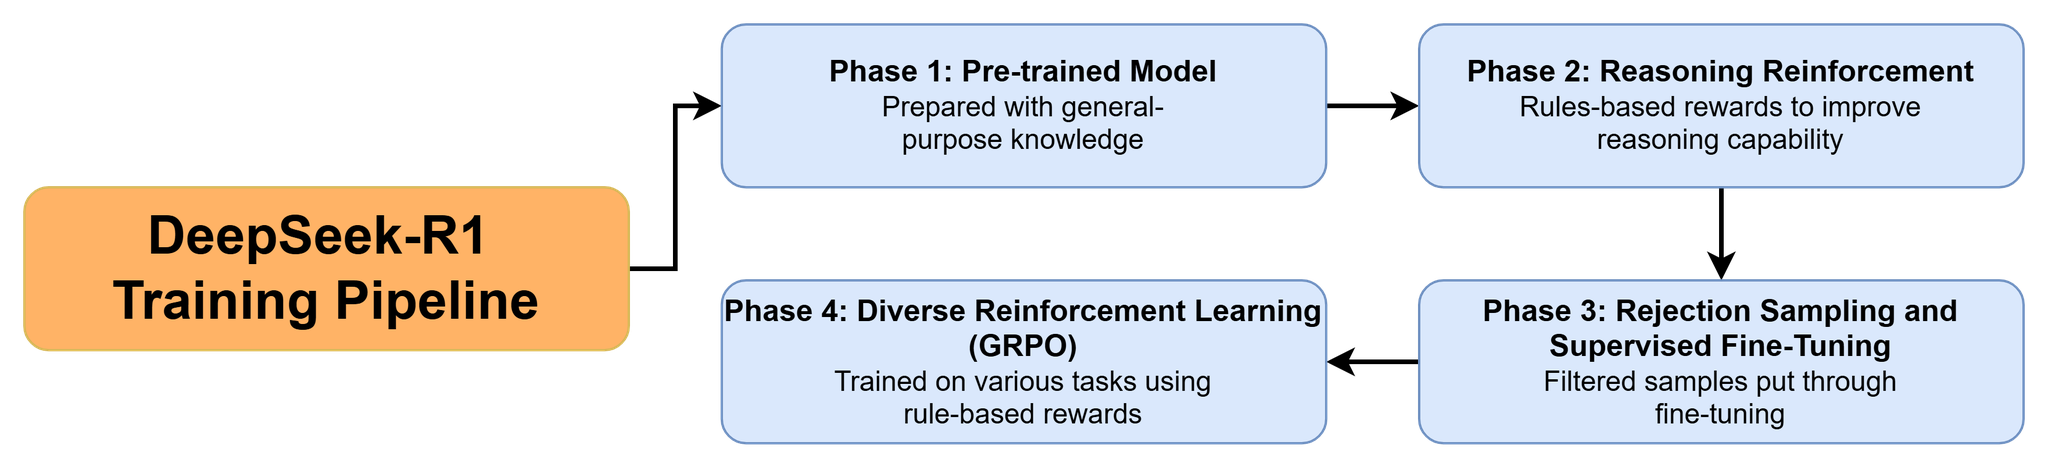
\includegraphics[width=0.7\textwidth]{figures/deepsek.png}
    \caption{DeepSeek-R1 Training Pipeline}
    \label{fig:deepseek_pipeline}
\end{figure}

While the DeepSeek-R1 model shown in Figure~\ref{fig:deepseek_pipeline} will serve as the generative backbone of the chatbot, this study will not involve the training of new LLMs. Instead, it will integrate the pre-trained model into an RAG framework to augment domain-specific information retrieval for CSPC Library users.

\section{Materials and Statistical Tools}

To ensure optimal performance of the RAG-based LLM system, several key hardware and software components are required.

\subsubsection*{Hardware}
\begin{table}[H]
    \centering
    \caption{Hardware Requirements}
    \label{tab:hardware_requirements}
    \begin{tabular}{ll}
        \hline
        \textbf{Component}       & \textbf{Specification}                     \\ \hline
        Processor (CPU)          & Modern Multi-core CPU                      \\
        Memory (RAM)             & 16 GB or higher                            \\
        Storage                  & 1 TB SSD or higher                         \\
        Graphics Card (GPU)      & NVIDIA RTX 3090+ (recommended)             \\
        \hline
    \end{tabular}
\end{table}

A modern multi-core CPU enables efficient data processing and model inference, ensuring smooth query execution. At least 16 GB of RAM is recommended to manage large-scale embeddings and real-time retrieval operations effectively. A 1 TB SSD is preferred due to its high read/write speeds, which significantly enhance data indexing and retrieval. Given the resource-intensive nature of embedding computations and AI-driven text generation, a high-performance GPU, such as an NVIDIA RTX 3090 or better, is crucial for accelerating deep learning inference and vector operations.


\subsubsection*{Software}

\begin{table}[H]
    \centering
    \caption{Software Requirements}
    \label{tab:software_requirements}
    \begin{tabular}{ll}
        \hline
        \textbf{Component}              & \textbf{Specification}                        \\ \hline
        Programming Language            & Python 3.10+                                  \\
        Vector Database                 & ChromaDB                                      \\
        Language Model                  & DeepSeek-R1                                   \\
        Embedding Model                 & DeepSeek Embedding                            \\
        Web Framework                   & Streamlit                                     \\
        Libraries                       & \begin{tabular}[c]{@{}l@{}}LangChain\\ PyMuPDF\\ NumPy\\ PyPDFLoader\end{tabular}   \\
        \hline
    \end{tabular}
\end{table}

Python 3.10 or later serves as the core programming language due to its comprehensive support for machine learning and natural language processing. ChromaDB is used as the vector database to facilitate fast and accurate semantic search. The system leverages DeepSeek-R1 (deployed locally via Ollama) as its LLM, which ensures data privacy during query generation. DeepSeek Embedding transforms preprocessed text chunks into semantically rich vector representations.

The Streamlit framework is used to build an interactive user interface, allowing seamless user interactions. Document parsing and extraction are managed through the PyMuPDF library, ensuring accurate and efficient retrieval of textual data from PDF files. NumPy supports numerical operations, while LangChain manages the orchestration of LLMs during query interpretation and response generation.

\section{Instruments}

The instruments that will be utilized in this study will include a curated dataset, a vector database, a user evaluation questionnaire, and an automated evaluation toolkit. The dataset will consist of all available PDF thesis documents sourced from the CSPC Library, which will be parsed using the PyMuPDF library for text extraction. These documents will undergo preprocessing, including cleaning and segmentation into manageable chunks, before being embedded using \textit{DeepSeek Embedding}, a modern embedding model known for its semantic richness and high compatibility with retrieval tasks.

The vectorized representations of these chunks will then be stored in \textit{ChromaDB}, an open-source vector database optimized for fast similarity search and retrieval, which is vital for the implementation of the RAGAS framework~\cite{trychroma2023chroma}.

To assess both technical and user-centered performance, multiple evaluation instruments will be employed. A user questionnaire will be used to gather feedback on usability, accuracy, and overall satisfaction, applying a 5-point Likert scale for consistent measurement.

Additionally, the RAGAS (Retrieval-Augmented Generation Assessment Suite) toolkit will be utilized to automatically evaluate the quality of system outputs using metrics such as \textbf{context precision}, \textbf{faithfulness}, and \textbf{answer relevance}~\cite{shinn2023ragas}. These instruments will ensure a rigorous and balanced evaluation of the proposed system from both system-level and user perspectives~ \cite{lin2021bert}.

\section{Statistical Tools}

The evaluation of the system will incorporate both descriptive and inferential statistical tools. Descriptive statistics such as \textit{mean} and \textit{standard deviation} will summarize user feedback, providing insight into central tendencies and variability in user experience~\cite{holmes2023chatbot}.

Additionally, \textbf{Cronbach’s Alpha} will be used to assess the internal consistency and reliability of the usability survey instrument. This coefficient measures whether the questionnaire items consistently reflect the intended construct of system usability, ensuring the validity of user feedback.

Finally, the RAGAS framework will be applied to evaluate the system's technical performance. It includes metrics such as \textit{context precision}, \textit{context recall}, and \textit{faithfulness}. These metrics will assess how accurately the system retrieves and utilizes relevant documents to generate responses~\cite{holmes2023chatbot, ameli2024ranking, lin2024satisfaction}.

\section{Procedures}

The procedures will encompass the collection and preprocessing of academic data, vector-based indexing, retrieval using semantic search, LLM-based response generation, and multi-metric evaluation using RAGAS.

Each stage is designed to ensure the integrity, replicability, and effectiveness of the system in addressing the research objectives. By detailing the technical and methodological steps, this section will serve as a transparent and structured guide for future researchers seeking to replicate or build upon this study.

\subsection*{Data Collection}
PDF thesis documents will be gathered from CSPC Library’s digital archives, focusing on undergraduate theses and institutional research. The collection process will ensure that documents are academically relevant and representative of typical user queries.

\subsection*{Data Preprocessing}
\begin{itemize}
    \item \textbf{Text Extraction:} PyMuPDF will be used to convert PDF files into structured plain text.
    \item \textbf{Cleaning:} Non-informative characters and formatting will be removed.
    \item \textbf{Text Chunking:} Text will be segmented into manageable chunks to enhance semantic search accuracy.
\end{itemize}

\subsection*{Indexing and Vector Embedding}
\begin{itemize}
    \item \textbf{Vector Embedding:} Each text chunk will be embedded using DeepSeek Embeddings.
    \item \textbf{Database Construction:} ChromaDB will store the vectorized content along with metadata such as document titles, authors, and section headers.
\end{itemize}

\subsection*{Query Handling and Semantic Retrieval}
\begin{itemize}
    \item \textbf{Query Encoding:} The user’s natural language query will be encoded using the same embedding model.
    \item \textbf{Similarity Search:} The encoded query will be matched with stored vectors to retrieve the top-K relevant chunks.
\end{itemize}

\subsection*{Augmented Input Generation}
The retrieved chunks will be concatenated with the user query to create an augmented prompt, providing contextual grounding for accurate response generation.

\subsection*{Response Generation}
The DeepSeek-R1 language model will process the augmented input to generate a response that is factually aligned with the source documents.

\subsection*{Output Presentation}
The system will display the generated response via a user interface that includes metadata such as the source thesis title and section, encouraging transparency and academic integrity.

\subsection*{Performance Evaluation}
\begin{itemize}
    \item \textbf{Automated Evaluation:} Metrics from the RAGAS framework, Context Precision, Context Recall, and Faithfulness, will be calculated.
    \item \textbf{Human Evaluation:} A usability questionnaire will be distributed to a sample of student users to assess the system’s clarity, ease of use, and usefulness in retrieving academic information.
\end{itemize}

\section{Evaluation Metrics}

\hspace{0.4cm}The researchers will use a framework called \textbf{RAGAS} that comprises specific metrics to assess Retrieval-Augmented Generation (RAG)-based architectures, thereby ensuring precise measurements of both retrieval quality and generation fidelity~\cite{oubah2024advanced}. This framework will evaluate the model's performance using the following metrics: \textbf{Context Precision}, \textbf{Context Recall}, and \textbf{Faithfulness}. Each metric is essential in addressing the system’s retrieval and generation performance.

\subsection*{Context Precision}

This metric evaluates the proportion of retrieved chunks that are relevant to the user’s query. A high context precision score in the CSPC Library RAG-based system indicates that the system retrieves thesis content closely aligned with student queries, ensuring efficient and meaningful academic assistance during literature searches.

% \begin{equation}
% \text{Precision@K} = \frac{1}{K} \sum_{k=1}^{K} v_k
% \end{equation}

\begin{figure}[H]
\centering
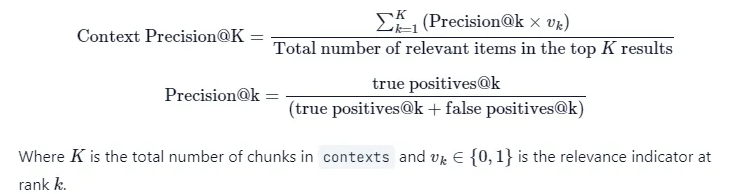
\includegraphics[width=0.7\textwidth]{figures/context_precision_formula.png}
\caption{Formula for Context Precision}
\label{fig:context_precision}
\end{figure}

\noindent Where:
\begin{itemize}
    \item $v_k \in \{0,1\}$ is the relevance indicator at rank $k$: $v_k = 1$ if the chunk at position $k$ is relevant; otherwise, $v_k = 0$.
    \item $K$ is the total number of retrieved chunks in the top-K results.
\end{itemize}

\subsection*{Context Recall}

Context Recall evaluates how effectively the system retrieves all relevant chunks from the dataset. This metric measures the proportion of relevant chunks successfully obtained, ensuring a comprehensive retrieval process that is essential for academic research tasks~\cite{danter2024advanced}.

% \begin{equation}
% \text{Recall} = \frac{\text{Number of reference claims supported by retrieved context}}{\text{Total number of reference claims}}
% \end{equation}

\begin{figure}[H]
\centering
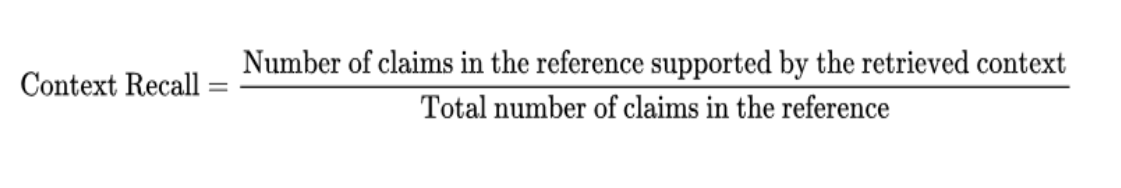
\includegraphics[width=0.7\textwidth]{figures/context_recall_formula.png}
\caption{Formula for Context Recall}
\label{fig:context_recall}
\end{figure}

\noindent Where:
\begin{itemize}
    \item \textbf{Number of claims in the reference supported by the retrieved context:} Total number of factual claims from the reference answer that appear in the retrieved chunks.
    \item \textbf{Total number of claims in the reference:} Total number of relevant factual claims that should ideally be retrieved to answer the query comprehensively.
\end{itemize}

\subsection*{Faithfulness}

Faithfulness assesses the factual accuracy and fidelity of the generated responses in relation to the retrieved content. It measures whether the generated answer remains grounded in the context retrieved from source documents~\cite{lin2024satisfaction}. In the CSPC Library RAG-based system, this ensures academic integrity and minimizes misinformation in automated answers.

% \begin{equation}
% \text{Faithfulness} = \frac{\text{Number of claims in response supported by retrieved context}}{\text{Total number of claims in response}}
% \end{equation}

\begin{figure}[H]
\centering
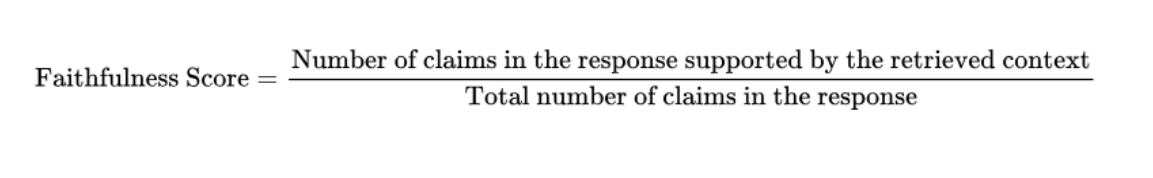
\includegraphics[width=0.7\textwidth]{figures/faithfulness_formula.png}
\caption{Formula for Faithfulness}
\label{fig:faithfulness}
\end{figure}

\noindent Where:
\begin{itemize}
    \item \textbf{Number of claims in the response supported by retrieved context:} The total number of claims in the response that can be directly inferred or verified from the retrieved context.
    \item \textbf{Total number of claims in the response:} The complete count of all claims made in the response, whether supported or unsupported by the context.
\end{itemize}

\section{Conceptual Framework}

The conceptual framework will serve as the foundational blueprint for the RAG-based chatbot system. It will emphasize the end-to-end interaction of modules required to support intelligent, accurate, and efficient academic document retrieval. As illustrated in Figure~\ref{fig:conceptual_framework}, the system will follow a cyclical process beginning with data collection and ending with system evaluation and refinement. In Figure~\ref{fig:conceptual_framework}, the arrows are used solely to visually indicate the step-by-step flow of each component within the chatbot framework; they do not signify any technical operation or special relationship beyond showing the direction of the process. This visualization helps guide readers through the sequence of the system stages, ensuring clarity at the outset.

\begin{figure}[H]
    \centering
    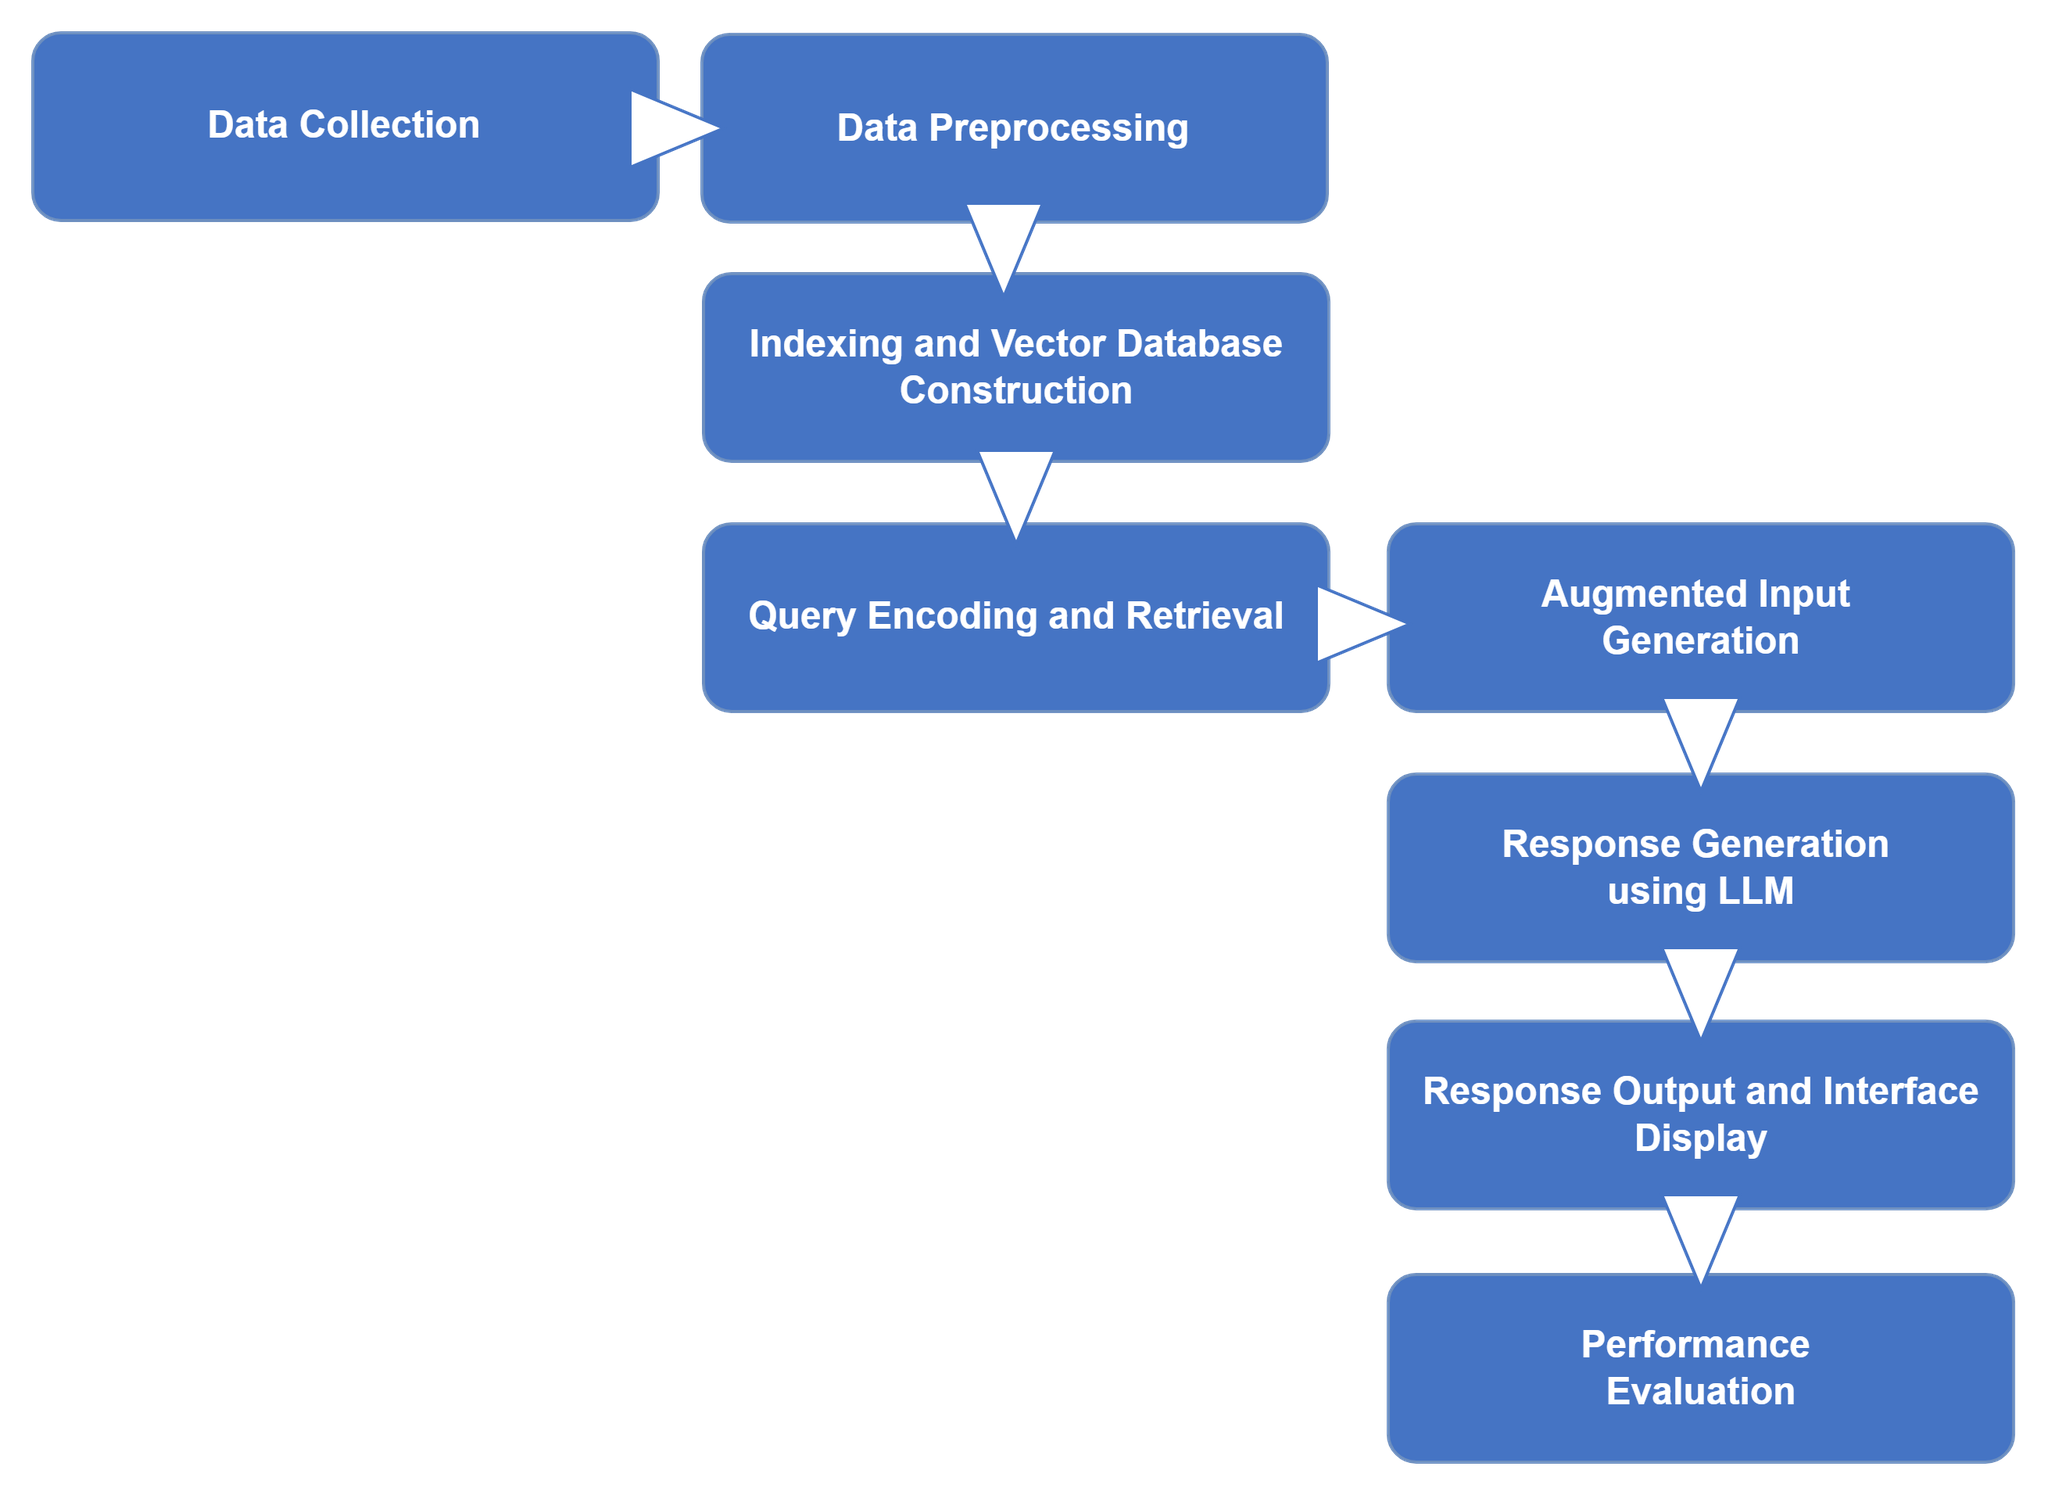
\includegraphics[width=0.7\textwidth]{figures/framework.png}
    \caption{Conceptual Framework of the RAG-Based Chatbot System}
    \label{fig:conceptual_framework}
\end{figure}

The process will begin with \textbf{data collection}, where PDF-format academic documents such as undergraduate theses and institutional research papers will be sourced from the CSPC Library’s digital repository. These documents will form the primary knowledge base of the system.

In the \textbf{data pre-processing} phase, tools like PyMuPDF will be used to extract plain text from the collected PDFs. The extracted content will undergo cleaning and normalization to remove non-informative characters, followed by segmentation into semantically meaningful text chunks.

Next, the system will perform \textbf{model training}, where embedding models such as DeepSeek Embeddings will be used to transform the text chunks into vector representations. These embeddings will preserve the semantic meaning of the documents and prepare them for storage and retrieval.

The \textbf{input sampling} stage will support the gathering and simulation of user queries. These sample inputs will reflect typical academic inquiries posed by students when searching for specific thesis content.

In the \textbf{input pre-processing} phase, user queries will be tokenized and encoded using the same embedding model applied during training. This will enable semantic similarity comparison between the user query and the pre-embedded document vectors.

The system will then proceed to \textbf{location mapping}, which will correspond to the semantic search function performed using ChromaDB. Here, the system will retrieve the top-K most relevant document chunks by measuring vector similarity.

During \textbf{model inference}, an augmented input will be created by combining the user query with the retrieved chunks. This augmented prompt will be forwarded to a generative language model (e.g., DeepSeek-R1) to produce a contextually grounded response aligned with the original academic documents.

Finally, \textbf{performance evaluation} will be conducted using a dual-layer assessment. System-level performance will be measured using the RAGAS framework with metrics such as Context Precision, Context Recall, and Faithfulness. In parallel, a user-centered evaluation will be carried out using a structured Likert-scale questionnaire to assess usability, relevance, and satisfaction.

This framework will ensure that each component of the RAG-based chatbot system will operate in coordination, contributing to a reliable and academically useful tool for thesis retrieval and literature assistance.

%=======================================================%
%%%%% Do not delete this part %%%%%%
\clearpage

\printbibliography[heading=subbibintoc, title={\centering Notes}]
\end{refsection}